%\documentclass[letterpaper, 10 pt, conference]{ieeeconf}
%pdflatex -synctex=1 -interaction=nonstopmode %.tex|makeindex %.glo -t %.glg -s %.ist -o %.gls|pdflatex -synctex=1 -interaction=nonstopmode %.tex|makeindex %.nmn -t %.nmg -s %.ist -o %.nmd|pdflatex -synctex=1 -interaction=nonstopmode %.tex|makeindex %.jmn -t %.jmg -s %.ist -o %.jmd|pdflatex -synctex=1 -interaction=nonstopmode %.tex|biber %|pdflatex -synctex=1 -interaction=nonstopmode %.tex|makeindex %.idx|pdflatex -synctex=1 -interaction=nonstopmode %.tex|pdflatex -synctex=1 -interaction=nonstopmode %.tex|"C:\Program Files\Adobe\Acrobat DC\Acrobat\Acrobat.exe" %.pdf
\documentclass[conference]{IEEEtran}

\usepackage{listings}
\usepackage{xcolor}
\usepackage{graphicx}
\usepackage{subfig}
\usepackage{tikz}
\usetikzlibrary{arrows.meta, positioning}
\usepackage{array}
\usepackage{float} % Requis pour l'option [H]
\usepackage{booktabs} % Pour des tableaux mieux formatés
\usepackage{placeins}

\usepackage[utf8]{inputenc}
\usepackage{amsmath}
\usepackage{amssymb}
\usepackage{balance}
\usepackage{cite}
\usepackage{fancyhdr}
\usepackage{lastpage} % Pour obtenir le nombre total de pages
\usepackage{stfloats}

\usepackage{algorithm}
\usepackage{algpseudocode} % Utilisé avec le package algorithm

\usepackage{url}
\usepackage{hyperref}
\usepackage{breakurl} % Pour gérer les retours à la ligne des URL

% Redéfinir le titre "Algorithm" en "Algorithme"
\floatname{algorithm}{Algorithme}
\renewcommand{\figurename}{Figure}
\renewcommand{\refname}{Bibliographie}
\renewcommand{\tablename}{Tableau}
\renewcommand{\thetable}{\arabic{table}}


% Configuration pour Python
\lstset{
    language=Python,
    basicstyle=\ttfamily\footnotesize,
    keywordstyle=\color{blue}\bfseries,
    stringstyle=\color{red},
    commentstyle=\color{green},
    breaklines=true,
    frame=single,
    numbers=left,
    numberstyle=\tiny,
    stepnumber=1,
    showspaces=false,
    showstringspaces=false,
    tabsize=4,
    captionpos=b
}

\IEEEoverridecommandlockouts                              
%\overrideIEEEmargins

\renewcommand\IEEEkeywordsname{Keywords}


\title{\LARGE \bf
CCF: Calcul Rapide et Évolutif des Composantes Connexes avec MapReduce
}

\author{
    \IEEEauthorblockN{Aurélien Duvignac-Rosa, Edoardo Piciucchi, Jean-Marc Fauvel}
}


\begin{document}

\pagestyle{fancy}
\fancyhf{}
\fancyfoot[C]{Page \thepage\ / \pageref{LastPage}}
\renewcommand{\headrulewidth}{0pt}
\renewcommand{\footrulewidth}{0pt}


\maketitle
\thispagestyle{empty}
\pagestyle{empty}


%%%%%%%%%%%%%%%%%%%%%% ABSTRACT %%%%%%%%%%%%%%%%%%%%%%%%%%%%%%%%%%%%
\begin{abstract}
Identifier les composantes connexes dans un graphe est un problème bien connu dans de nombreux domaines d'application tels que l'analyse des réseaux sociaux, l'exploration de données, le traitement d'images, et bien d'autres encore.
Ce projet porte sur l'étude de \cite{6785473}, qui vise à identifier toutes les composantes connexes dans un graphe donné à l'aide du paradigme \textit{MapReduce}.
Notre implémentation s'est faite exclusivement en \textit{pyspark}.
Nous présenterons tout d'abord notre implémentation de l'algorithme \textit{CCF} appliqué à deux structures de données : les \textit{RDD} (\textit{Resilient Distributed Dataset}) et \textit{DataFrame} pour ensuite appliquer notre implémentation sur le graphe fourni dans l'article \cite{6785473} et enfin étendre notre travail sur des graphes beaucoup plus importants afin de mener une étude comparative entre les deux structures de données exploitées et les algorithmes étudiés.
\end{abstract}
\begin{IEEEkeywords}
Composantes connexes ; Graphes à grande échelle ; PySpark ; MapReduce.
\end{IEEEkeywords}
%%%%%%%%%%%%%%%%%%%%%% ABSTRACT %%%%%%%%%%%%%%%%%%%%%%%%%%%%%%%%%%%%

\section{Introduction}
\cite{6785473} propose un algorithme de calcul de composantes connexes en utilisant le modèle de programmation \textit{MapReduce}, basé sur l'algorithme de \textit{Label Propagation} et conçu pour être rapide et extensif (\textit{scalable}), c'est-à-dire pouvant être utilisé sur de grands ensembles de données et un grand nombre de machines.

L'algorithme a pour objectif d'identifier les sous-graphes connectés au sein d'un graphe $G$. Ce dernier devant être représenté par une collection de paires $(N_{1}, N_{2})$ où $N_{1}$ et $N_{2}$ sont des nœuds du graph $G$ qui ont une connexion entre eux. Le couple $(N_{1}, N_{2})$ représentant une arête du graphe.

L'algorithme décrit dans \cite{6785473} identifie les sous-graphes connectés en transformant leurs paires sous la forme $(N, N_{min})$, où $N$ est un nœud et $N_{min}$ le nœud de plus petite valeur du même sous-graphe. Conçu pour traiter de grands graphes, il utilise une programmation distribuée basée sur \textit{MapReduce}, permettant de paralléliser le traitement sur plusieurs machines.

\section{Objectifs du projet}
\begin{enumerate}
    \item Lire, comprendre et expliquer l'algorithme décrit dans \cite{6785473} ;
    \item Coder l'algorithme en \textit{Spark} en utilisant à la fois des \textit{RDD} (\textit{Resilient Distributed Dataset}) et \textit{DataFrame} ;
    \item L'implémentation doit être exécutée en Python, et optionnellement en \textit{Scala} ;
    \item Effectuer une analyse comparative des versions en \textit{RDD} et \textit{DataFrame} sur des graphes de tailles croissantes ;
    \item Utilisation de \textit{DataBricks}\footnote{L'ensemble des graphiques présentés dans ce document ont été obtenus par \textit{DataBricks}} pour les petits graphes, et \textit{Google Cloud Cluster} pour les plus gros ($<$ 20 Gb).
\end{enumerate}

\section{Présentation de l'algorithme CCF}

L'algorithme \textit{CCF}, présenté dans \cite{6785473}, se décompose en trois sous algorithmes distincts : \textit{CCF-Iterate}, \textit{CCF-Dedup} et une optimisation : \textit{CCF (secondary sorting)}, chacun respectivement rappelé dans les algorithmes de ce document \ref{alg:ccf_iterate}, \ref{alg:ccf_dedup} et \ref{alg:ccf_iterate_secondary_sorting}. Ces derniers ont été étudiés et implémentés en \textit{pyspark}.

\begin{minipage}[t]{0.48\textwidth} % Limitation à une colonne
\tiny % Réduction de la taille de l'algorithme
\begin{algorithm}[H]
\caption{CCF-Iterate}
\label{alg:ccf_iterate}
\begin{algorithmic}[1]
    \Function{Map}{\textit{key}, \textit{value}}
        \State \textbf{emit}(\textit{key}, \textit{value})
        \State \textbf{emit}(\textit{value}, \textit{key})
    \EndFunction
    \Function{Reduce}{\textit{key}, \textit{values}}
        \State \textit{min} $\gets$ \textit{key}
        \For{\textit{value} $\in$ \textit{values}}
            \If{\textit{value} $<$ \textit{min}}
                \State \textit{min} $\gets$ \textit{value}
            \EndIf
            \State \textit{valueList.add}(\textit{value})
        \EndFor
        \If{\textit{min} $<$ \textit{key}}
            \State \textbf{emit}(\textit{key}, \textit{min})
            \For{\textit{value} $\in$ \textit{valueList}}
                \If{\textit{value} $\neq$ \textit{min}}
                    \State \textit{Counter.NewPair.increment(1)}
                    \State \textbf{emit}(\textit{value}, \textit{min})
                \EndIf
            \EndFor
        \EndIf
    \EndFunction
\end{algorithmic}
\end{algorithm}
\end{minipage}
\hfill
\begin{minipage}[t]{0.48\textwidth} % Limitation à une colonne
\tiny % Réduction de la taille de l'algorithme
\begin{algorithm}[H]
\caption{CCF-Dedup}
\label{alg:ccf_dedup}
\begin{algorithmic}[1]
    \Function{Map}{\textit{key}, \textit{value}}
        \State \textit{temp.entity1} $\gets$ \textit{key}
        \State \textit{temp.entity2} $\gets$ \textit{value}
        \State \textbf{emit}(\textit{temp}, \textit{null})
    \EndFunction
    \\
    \Function{Reduce}{\textit{key}, \textit{values}}
        \State \textbf{emit}(\textit{key.entity1}, \textit{key.entity2})
    \EndFunction
\end{algorithmic}
\end{algorithm}
\end{minipage}

\balance % Équilibre le contenu des colonnes

\newpage

\begin{minipage}[t]{0.48\textwidth} % Limitation à une colonne
\tiny % Réduction de la taille de l'algorithme
\begin{algorithm}[H]
\caption{CCF-Iterate (with secondary sorting)}
\label{alg:ccf_iterate_secondary_sorting}
\begin{algorithmic}[1]
    \Function{Map}{\textit{key}, \textit{value}}
        \State \textbf{emit}(\textit{key}, \textit{value})
        \State \textbf{emit}(\textit{value}, \textit{key})
    \EndFunction
    \Function{Reduce}{\textit{key}, \textit{values}}
        \State \textit{minValue} $\gets$ \textit{values.next()}
        \If{\textit{minValue} $<$ \textit{key}}
            \State \textbf{emit}(\textit{key}, \textit{minValue})
        \EndIf
        \For{\textit{value} $\in$ \textit{values}}
            \State \textit{Counter.NewPair.increment(1)}
            \State \textbf{emit}(\textit{value}, \textit{minValue})
        \EndFor
    \EndFunction
\end{algorithmic}
\end{algorithm}
\end{minipage}



\subsection{Explication des sous algorithmes}

\begin{itemize}
\item \textit{CCF-iterate} : cette étape consiste à propager les étiquettes des composants en mettant à jour chaque nœud avec la plus petite étiquette disponible. Le processus se répète jusqu'à stabilisation des étiquettes ;
\item \textit{CCF-dedup} : Cette étape consiste à supprimer les arêtes redondantes pour réduire le graphe et éviter des calculs inutiles ;
\item \textit{CCF-iterate (with secondary sorting)}, une variante de l'algorithme \textit{CCF-iterate}, optimise l'utilisation de la mémoire en éliminant la nécessité de rechercher la valeur minimale dans un groupe de nœuds connectés.
\end{itemize}

\subsection{Présentation de l'algorithme pas à pas}

\begin{itemize}
\item \textbf{données d'entrées} : paires de nœuds $(N_{1}, N_{2})$, représentant les arêtes du graphe, stockées sous forme d'un graphe noté $G = (V, E)$ avec $V$ (\textit{vertices}), les sommets et $E$ (\textit{edges}), les arêtes.
\item \textbf{données de sortie} : paires de nœuds $(N_{i}, N_{min})$ où $N_{i} \; \forall i \in [0;n]_{\mathbb{N}}$, $n$ étant le nombre de noeud du graphe complet, est un nœud du sous-graphe et $N_{min}$ est le nœud de plus petite valeur appartenant au même sous-graphe. Ces paires sont stockées sous forme d'un graphe noté $G' = (V', E')$ avec $V'$ les sommets et $E'$ les arêtes.
\end{itemize}

\balance % Équilibre le contenu des colonnes

\subsection{Implémentation de l'algorithme \textit{CCF} en paradigme \textit{Spark}}

L'implémentation décrite fournie dans le \textit{notebook} associé permet de réaliser les étapes de l'algorithme \textit{CCF} décrites dans l'exemple de \cite{6785473}. Les résultats obtenus nous ont permis de constater une erreur au niveau de l'exemple de \cite{6785473}. En effet, dans la figure 5.1 de \cite{6785473}, bien que H $>$ G, l'arête H $\rightarrow$ G n'est pas transmise dans le graphe de la colonne \textit{Reducer} lors de la première itération, ce qui propage une erreur à chaque itération. Cependant, le résultat final reste correct.

Pour le prouver, il suffit d'instancier le paramètre \textit{debug} à \textit{True} dans la méthode \textit{workflow} décrite dans le code fourni. Cela permet d'afficher les graphes successifs obtenus après chaque itération de l'algorithme.

L'implémentation s'est faite en s'appuyant sur la programmation orientée objet : permettant ainsi de réduire au maximum la redondance de code et ainsi en assurer une meilleure lisibilité. Les deux structures de données \textit{RDD} et \textit{DataFrame} ont été encapsulées dans deux classes distinctes : \textit{GraphRDD} et \textit{GraphDF} elle-mêmes héritant d'une classe mère \textit{Graph} qui implémente à la fois les méthodes abstraites requises comme \textit{reducer} et \textit{mapper} mais également des méthodes communes comme \textit{ccf-iterate} et \textit{workflow} : en charge d'exécuter le \textit{workflow} complet de l'algorithme de recherche de composantes connexes.
De plus, l'algorithme \textit{CCF-Iterate (secondary sorting)} (cf. algorithme \ref{alg:ccf_iterate_secondary_sorting}), présenté dans \cite{lin2010data} a été implémenté par l'intermédiaire de deux autres classes : \textit{Graph\_RDD\_Secondary\_Sorting} et \textit{Key1Partitioner}.

\section{Présentation des résultats obtenus}

Les résultats obtenus, présentés dans la figure \ref{fig:exec_time_vs_nb_edges_input} et le tableau \ref{tab:summary_results}, ont permis de mettre en exergue deux points importants.
D'une part, comme en témoignent la figure \ref{subfig:exec_time_vs_nb_edges_input_reg_lineaire_exponentielle} et le tableau \ref{tab:summary_results}, la structure de données \textit{RDD} est beaucoup plus \textit{résiliente} et permet une \textit{scalabilité} sur des graphes de très grandes tailles à la différence de la structure \textit{DataFrame} qui ne fournit pas un temps de traitement aussi faible que les \textit{RDD}.
Les points bleus (resp. rouges) de la figure \ref{subfig:exec_time_vs_nb_edges_input_reg_lineaire_exponentielle}, représentent les temps d'exécution successifs pour les \textit{RDD} avec l'algorithme \textit{CCF} (resp. \textit{CCF with secondary sorting}), montrent une croissance quasi-linéaire, confirmée par les lignes d'ajustement linéaire (pointillées). Cela indique que les \textit{RDD} sont extrêmement efficaces et leur \textit{scalabilité} est quasi constante, même pour des graphes de grande taille.
Quant aux temps d'exécution des \textit{DataFrames}, représentés par les points verts, deux éléments notables peuvent s'en dégager :
\begin{enumerate}
\item une croissance linéaire est à noter dans les premières étapes ;
\item Une tendance exponentielle qui se manifeste pour des graphes de grande taille, confirmée par l'ajustement exponentiel
\end{enumerate}
Cela reflète un comportement beaucoup moins efficace et une incapacité à traiter efficacement des graphes de taille croissante.
Cette divergence de comportement provient du fait que les \textit{RDD} sont conçus pour un traitement distribué natif et exploitent mieux les capacités du système distribué (parallélisme, partitionnement, résilience).
Tandis que les \textit{DataFrames}, bien que plus optimisés pour des cas de calcul spécifiques, nécessitent des surcoûts liés à la gestion des métadonnées et aux optimisations internes, ce qui peut engendrer des ralentissements pour des charges de travail très importantes.
La tendance exponentielle observée pour les \textit{DataFrames} peut s'expliquer par une gestion inefficace de la mémoire et des ressources au fur et à mesure que la taille des graphes augmente.
La surcharge d'optimisation et la gestion des partitions deviennent des goulets d'étranglement, entraînant une explosion des temps de calcul.

D'autre part, la figure \ref{subfig:exec_time_vs_nb_edges_input_reg_lineaire_exponentielle_RDD_uniquement_Databricks} démontre que l'efficacité de l'algorithme de \textit{secondary sorting} n'a pu être mis en évidence avec les \textit{datasets} fournis (cf. \cite{email_eu_core,ca_grqc,facebook_combined,ca_condmat,email_enron,cit_hepph}). Ces résultats sont corroborés par \cite{6785473} et \cite{databricks_url} qui indiquent que malgré des graphes très conséquents, ces derniers sont trop petits pour observer une amélioration significative du temps d'exécution. Des tailles de plusieurs millions d'arêtes sont nécessaires.

\begin{minipage}[t]{\columnwidth}
\centering
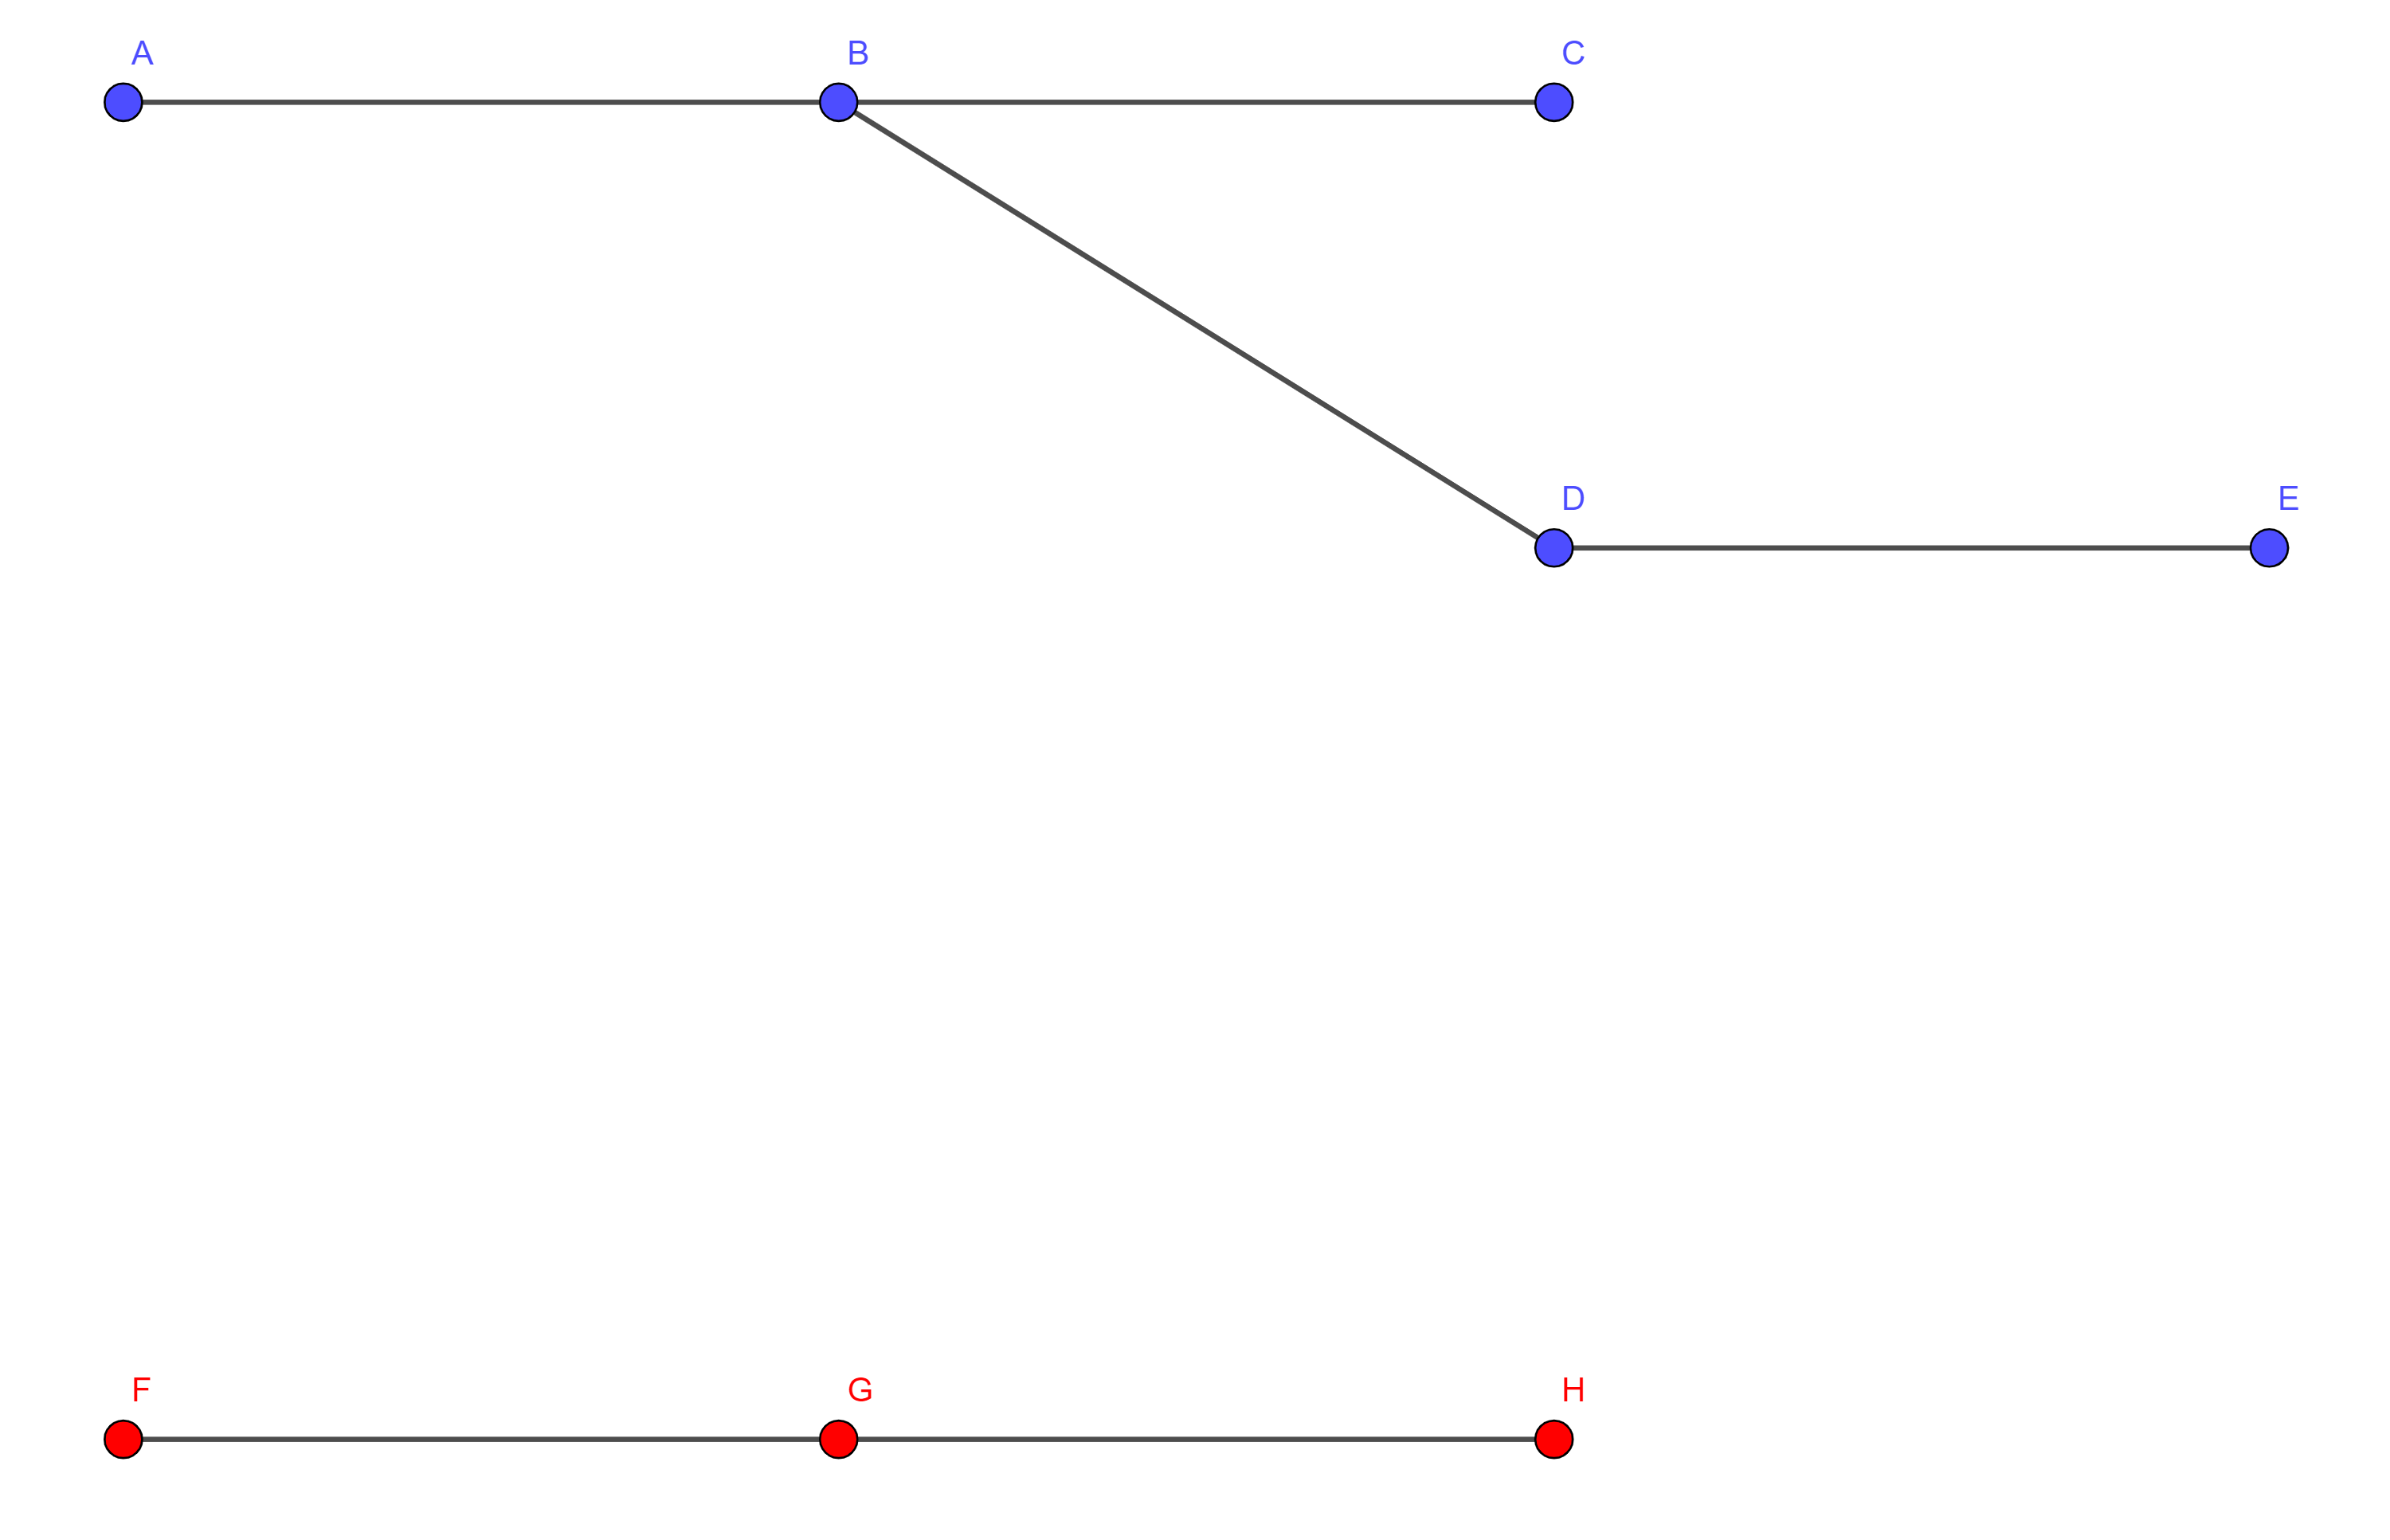
\includegraphics[scale=0.8]{figures/graphe_exemple.png}
\captionof{figure}{Graphe issu de \cite{6785473}.}
\label{fig:graphe_exemple}
\end{minipage}

\begin{figure*}[htbp]
    \centering
%    \subfloat[Démonstration (0 et 6 arêtes).]{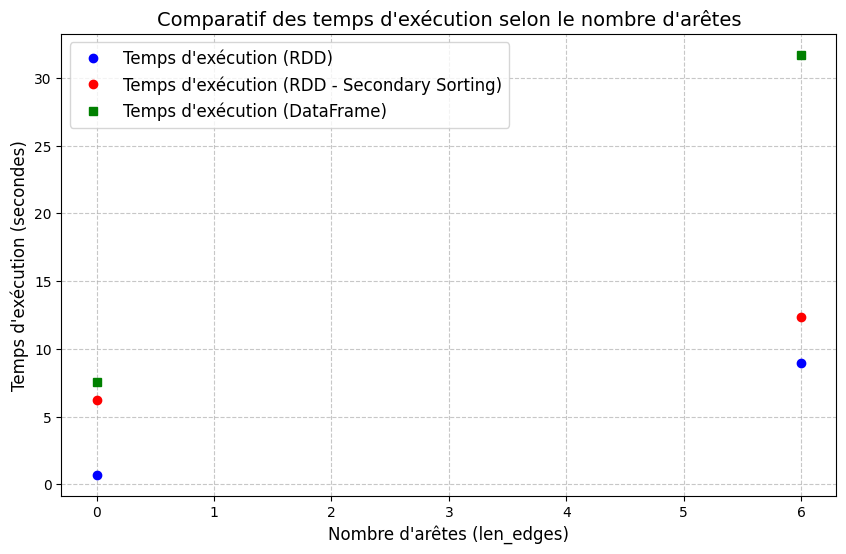
\includegraphics[width=0.48\linewidth]{figures/exec_time_vs_nb_edges_input_demo.png}\label{subfig:exec_time_vs_nb_edges_input_demo}}
%    \hfill
%    \subfloat[\textit{Dataset} complet.]{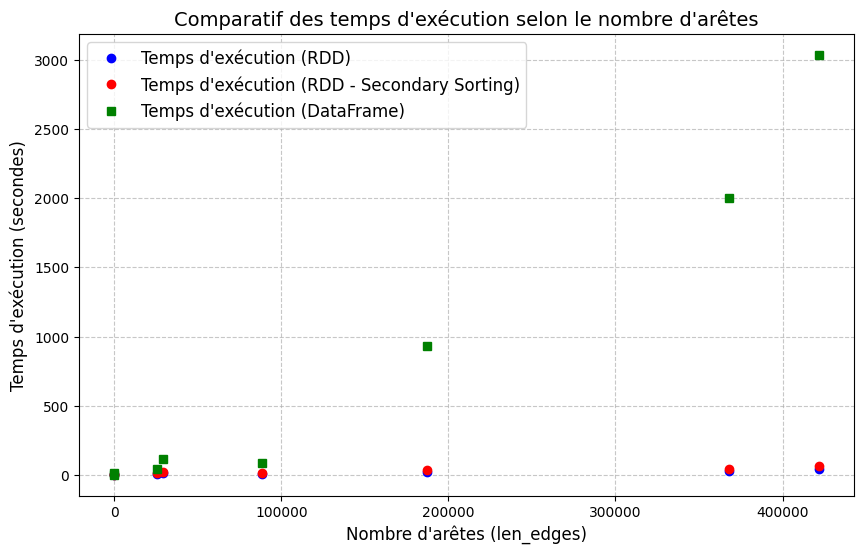
\includegraphics[width=0.48\linewidth]{figures/exec_time_vs_nb_edges_input.png}\label{subfig:exec_time_vs_nb_edges_input}}
%    \vspace{0.3cm} % Espacement vertical entre les lignes de sous-figures
%    \hfill
    \subfloat[\textit{Dataset} complet avec régression linéaire et exponentielle.]{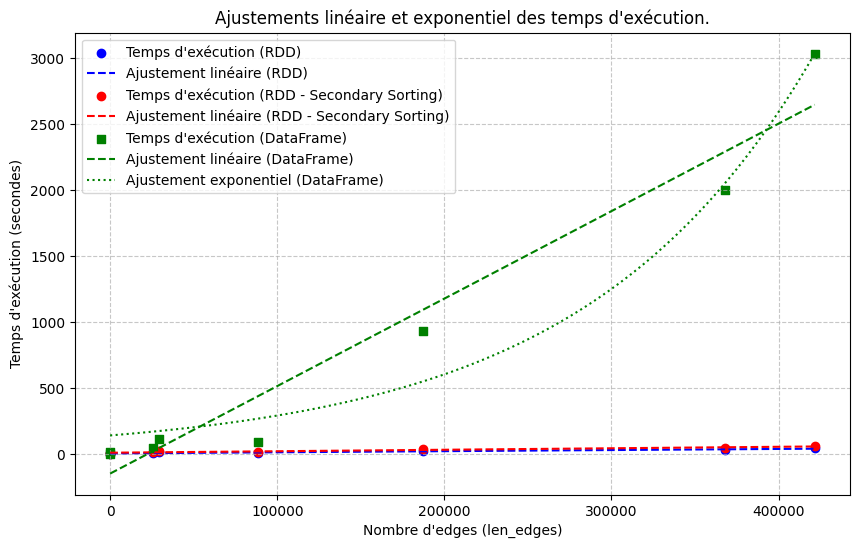
\includegraphics[width=0.48\linewidth]{figures/exec_time_vs_nb_edges_input_reg_lineaire_exponentielle.png}\label{subfig:exec_time_vs_nb_edges_input_reg_lineaire_exponentielle}}
    \hfill
    \subfloat[\textit{Dataset} complet avec régression linéaire (\textit{RDD} et \textit{RDD secondary sorting}).]{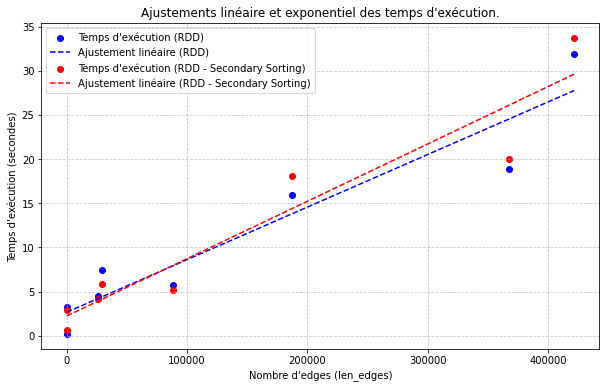
\includegraphics[width=0.48\linewidth]{figures/exec_time_vs_nb_edges_input_reg_lineaire_exponentielle_RDD_uniquement_Databricks.png}\label{subfig:exec_time_vs_nb_edges_input_reg_lineaire_exponentielle_RDD_uniquement_Databricks}}
    
    \caption{Comparatif des temps d'exécution en fonction du nombre d'arêtes d'entrée.}
    \label{fig:exec_time_vs_nb_edges_input}
\end{figure*}

\section{Garantie de l'intégrité des résultats obtenus}

Pour garantir l'intégrité des résultats, une analyse minutieuse des éléments de \textit{debug} du graphe fourni dans \cite{6785473}, illustré par la figure \ref{fig:graphe_exemple}, a été menée. De plus, après chaque traitement d'un jeu de données, une comparaison des résultats obtenus pour chaque structure de données a été réalisée (cf. tableau \ref{tab:summary_results}). En effet, nous avons faits l'hypothèse que si le nombre d'itération, le nombre de \textit{clusters} obtenus, et les éléments relatifs à chaque \textit{cluster} sont identiques pour l'ensemble des structures de données exploitées, et \textit{a fortiori} des classes et des méthodes implémentées, les résultats sont correctes.

\begin{minipage}[t]{\columnwidth}
\centering
\tiny
\captionof{table}{Résumé des résultats pour différents \textit{datasets} et structures de données.}
\label{tab:summary_results}
\begin{tabular}{@{}llcccc@{}}
\toprule
\textbf{\textit{dataset}} & \textbf{SDD} & \textbf{nb d'arêtes d'entrée} & \textbf{Temps d'exécution (s)} & \textbf{itérations} & \textbf{\textit{clusters}} \\ \midrule
Vide & RDD & 0 & 0.190470 & 1 & 0 \\
Vide & RDD Secondary Sorting & 0 & 0.678277 & 1 & 0 \\
Vide & Dataframe & 0 & 1.883 & 1 & 0 \\
\cite{6785473} & RDD & 6 & 3.230718 & 4 & 2 \\
\cite{6785473} & RDD Secondary Sorting & 6 & 2.885972 & 4 & 2 \\
\cite{6785473} & Dataframe & 6 & 14.630 & 4 & 2 \\
\cite{email_eu_core} & RDD & 25571 & 4.538241 & 5 & 1 \\
\cite{email_eu_core} & RDD Secondary Sorting & 25571 & 4.197027 & 5 & 1 \\
\cite{email_eu_core} & Dataframe & 25571 & 45.649 & 5 & 1 \\
\cite{ca_grqc} & RDD & 28980 & 7.400668 & 7 & 354 \\
\cite{ca_grqc} & RDD Secondary Sorting & 28980 & 5.816829 & 7 & 354 \\
\cite{ca_grqc} & Dataframe & 28980 & 111.948 & 7 & 354 \\
\cite{facebook_combined} & RDD & 88234 & 5.781553 & 5 & 1 \\
\cite{facebook_combined} & RDD Secondary Sorting & 88234 & 5.156801 & 5 & 1 \\
\cite{facebook_combined} & Dataframe & 88234 & 89.160 & 5 & 1 \\
\cite{ca_condmat} & RDD & 186936 & 15.948345 & 7 & 567 \\
\cite{ca_condmat} & RDD Secondary Sorting & 186936 & 18.105718 & 7 & 567 \\
\cite{ca_condmat} & Dataframe & 186936 & 929.319 & 7 & 567 \\
\cite{email_enron} & RDD & 367662 & 18.921314 & 6 & 1065 \\
\cite{email_enron} & RDD Secondary Sorting & 367662 & 19.994005 & 6 & 1065 \\
\cite{email_enron} & Dataframe & 367662 & 2004.748 & 6 & 1065 \\
\cite{cit_hepph} & RDD & 421578 & 31.950516 & 7 & 61 \\
\cite{cit_hepph} & RDD Secondary Sorting & 421578 & 33.771847 & 7 & 61 \\
\cite{cit_hepph} & Dataframe & 421578 & 3036.168 & 7 & 61 \\ \bottomrule
\\ \bottomrule
\end{tabular}
\end{minipage}

\section{Analyse quantitative sur l'utilisation de mémoire de \textit{RDD} et \textit{RDD secondary sorting}}

La figure \ref{subfig:exec_time_vs_nb_edges_input_reg_lineaire_exponentielle_RDD_uniquement_Databricks} ne permettant pas de mettre en évidence de manière significative l'impact du tri secondaire sur le temps d'exécution, nous avons formulé l'hypothèse que son principal avantage résidait dans la réduction de la mémoire utilisée. Pour valider cette hypothèse, notre première approche a consisté à analyser la mémoire consommée en fonction du nombre d'arêtes en entrée. Cependant, nous avons été confrontés au problème du \textit{Garbage Collector} de \textit{PySpark}, qui, étant déclenché après chaque traitement, entraînait des valeurs négatives de mémoire utilisée et une forte variabilité des résultats, empêchant ainsi toute validation concluante, comme illustré par la figure \ref{subfig:memory_vs_nb_edges_epoch_1}.

Pour surmonter cette difficulté, nous avons répété dix fois le traitement des \textit{datasets} pour les classes \textit{RDD} et \textit{RDD\_secondary\_sorting}, permettant ainsi de lisser les fluctuations dues au \textit{Garbage Collector} et d'obtenir une tendance cohérente et croissante de la mémoire utilisée en fonction du nombre d'arêtes en entrée. Cette approche nous a permis d'obtenir la figure \ref{subfig:memory_vs_nb_edges_epoch_10}, offrant une représentation plus fidèle de l'évolution de la mémoire consommée.

\newpage

\begin{figure*}[htbp]
    \centering
    \subfloat[Quantité de mémoire utilisée selon \textit{RDD} et \textit{RDD secondary sorting} (1 epoch).]{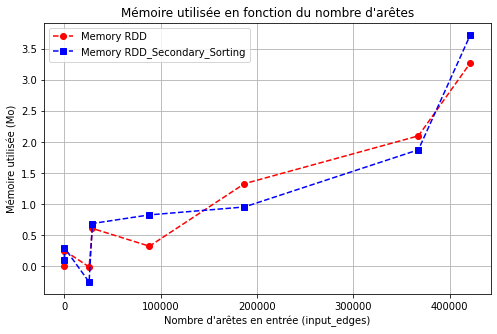
\includegraphics[width=0.48\linewidth]{figures/memory_vs_input_edges_epoch_1.png}\label{subfig:memory_vs_nb_edges_epoch_1}}
    \hfill
    \subfloat[Quantité de mémoire utilisée selon \textit{RDD} et \textit{RDD secondary sorting} (10 epoch).]{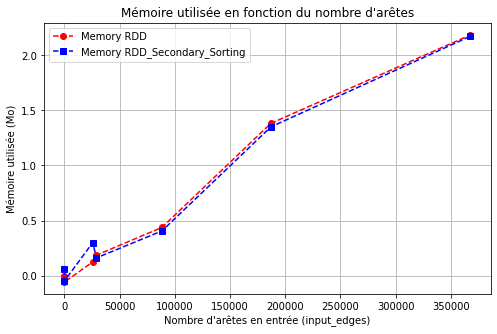
\includegraphics[width=0.48\linewidth]{figures/memory_vs_input_edges_epoch_10.png}\label{subfig:memory_vs_nb_edges_epoch_10}}
    \caption{Comparatif de la quantité de mémoire utilisée en fonction du nombre d'arêtes d'entrée.}
    \label{fig:memory_vs_nb_edges_input}
\end{figure*}

\section{Conclusion}

Ce travail a permis d'étudier et d'implémenter l'algorithme \textit{Connected Components Finder (CCF)}, basé sur le paradigme \textit{MapReduce}, pour identifier les composantes connexes dans un graphe. L'implémentation a été réalisée en \textit{pyspark} avec deux structures de données distinctes: \textit{RDD} et \textit{DataFrame}, afin de comparer leurs performances sur des graphes de tailles croissantes.

Les résultats obtenus montrent que les \textit{RDD} offrent des performances bien supérieures aux \textit{DataFrames} en termes de \textit{scalabilité} et de temps d'exécution. En effet, les \textit{RDD} présentent une croissance quasi-linéaire des temps d'exécution, même sur des graphes de très grande taille, grâce à leur conception native pour le traitement distribué et leur gestion efficace des partitions. À l'inverse, les \textit{DataFrames} affichent une croissance exponentielle des temps d'exécution pour les graphes plus grands, en raison de la surcharge liée à la gestion des métadonnées et des ressources.

Par ailleurs, l'optimisation par tri secondaire (secondary sorting) appliquée aux RDD n'a pas montré de gains significatifs sur les graphes testés, probablement en raison de leur taille insuffisante pour exploiter pleinement cette approche. Toutefois, cette technique pourrait se révéler bénéfique pour des graphes contenant plusieurs millions d'arêtes. Bien que le temps d'exécution soit souvent plus élevé, l'hypothèse selon laquelle le tri secondaire réduit l'empreinte mémoire a été confirmée, malgré des courbes de consommation de mémoire très proches entre la méthode classique et cette optimisation.

En conclusion, ce travail met en évidence l'intérêt d'utiliser les \textit{RDD} pour des graphes de grande taille en raison de leur résilience et de leur \textit{scalabilité}, tandis que les \textit{DataFrames} montrent des limitations importantes pour ces cas d'usage. Ces résultats ouvrent la voie à des travaux futurs portant sur l'optimisation des \textit{DataFrames} ou l'application de ces implémentations à des graphes de taille encore plus importante.

\bibliographystyle{IEEEtran}
\bibliography{bibliography} % Nom du fichier .bib sans l'extension

\balance % Équilibre le contenu sur les deux colonnes

\end{document}